\documentclass[11pt]{article}
\usepackage[toc,page]{appendix}
\usepackage{amsmath, amssymb}
\usepackage[utf8]{inputenc}
\usepackage[T1]{fontenc}
\usepackage[style=apa,backend=biber]{biblatex}
%\usepackage{biblatex}
\addbibresource{references.bib}
\usepackage{graphicx}
\usepackage{tikz}
\usetikzlibrary{automata,positioning,shapes.geometric, arrows.meta, fit, backgrounds, calc, chains}
\graphicspath{./images/Easy_Pictures/SMR_MULT_Repackaging}%\usepackage{kpfonts}
\usepackage{float}
\usepackage[margin=1in]{geometry}
\usepackage{cancel}
\usepackage{epsfig}
\usepackage{tikz-3dplot}
\usepackage{darkmode}
\usepackage{dirtytalk}
\usepackage{longtable,booktabs,array}
\usepackage{calc} % for calculating minipage widths
\usepackage[utf8]{inputenc}
\usepackage[T1]{fontenc}
\usepackage{xcolor}
\usepackage{listings}


\usepackage{etoolbox}
\usepackage{hyperref}
\hypersetup{
    colorlinks=true,
    linkcolor=blue,
    filecolor=magenta,      
    urlcolor=cyan,
    pdftitle={Hermeneutic Calculator},
    citecolor=blue,
    }


\urlstyle{same}

\lstdefinestyle{htmlStyle}{
    language=HTML,
    basicstyle=\ttfamily\small,
    keywordstyle=\color{blue}\bfseries,
    commentstyle=\color{gray}\itshape,
    stringstyle=\color{red},
    breaklines=true,
    frame=single,
    numbers=left,
    numberstyle=\tiny\color{gray},
    columns=fullflexible,
}
\lstdefinelanguage{HTML}{
  keywords={<!DOCTYPE, html, head, title, body, h1, h2, h3, p, div, span, a, img, ul, li, table, tr, td, th, style, link, script},
  sensitive=true,
  comment=[l]{//},
  morecomment=[s]{/*}{*/},
  morestring=[b]',
  morestring=[b]"
}
\lstset{style=htmlstyle, language=html}
% Updated to explicitly pass the language option
%\lstinputlisting[style=htmlstyle, language=html]{./html/example.html}
%\usepackage{tocloft}

% Optional: define some custom colors
\definecolor{sliceRed}{RGB}{225,224,91} % matching "varyellow" from your code
\definecolor{linkYellow}{RGB}{255,215,0}  % a golden yellow
\tdplotsetmaincoords{70}{110}

\title{Addition Strategies: Chunking by Bases and Ones}
\author{Compiled by: Theodore M. Savich}


\begin{document}
\maketitle
\subsection*{Transcript}
Strategy descriptions and examples adapted from \textcite{HackenbergCourseNotes}. Problem: Max  has  46  comic  books. For  his  birthday,  his  father  gives him  37  more  comic  books. How  many  comic  books  does  Max  have  now? 

\textbf{Dionne's solution:} ``He has 46. Then 37 more. {[}She writes
down 46, 76.{]} That's the 30. And then 7 more. Well, 4 more makes 80,
and then I only need to do 3 more, 83.''


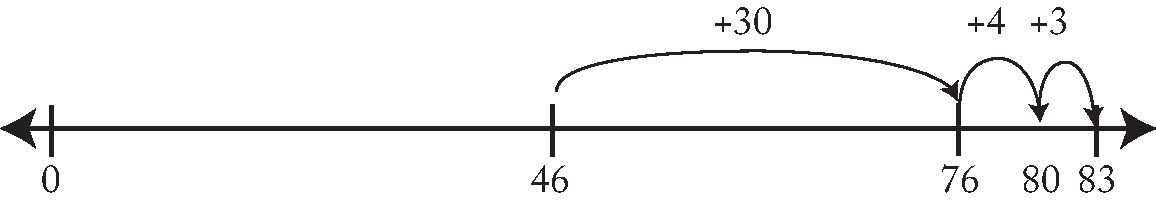
\includegraphics[width=.8\textwidth]{images/Easy_Pictures/SAR_ADD_CHUNKING/PDF/SAR_ADD_CHUNKING.pdf}

\noindent \textbf{Notation Representing Sarah's Solution:}

\begin{align*}
46 + 37 &= \Box \\
46 + 30 &= 76\\
76 + 4  &= 80\\
80+3 &= 83
\end{align*}

\subsubsection*{Description of Strategy:}

 \textbf{Objective:} Begin with one number. Then, break the other number down into bases and units. In COBO, you count on each base individually - then the ones. With Chunking, instead of adding each base individually, add them in well-chosen, larger groups. Likewise, combine the units in groups rather than one by one—though there are instances when adding a single base or unit makes strategic sense. The overall goal is to create larger, intentional groupings, and it’s important to clarify why each grouping is considered strategic. Usually, the goal with chunking on ones is to make a base first, then you can chunk on the rest of the ones. Usually when chunking on the bases, the goal is to make a base-of-bases first (so, in base ten, the goal would be to try and make one hundred), because then you can chunk on the rest of the bases (and ones) all at once. 

\subsubsection*{Description of Strategy}
\begin{itemize}
    \item \textbf{Objective:} Similar to COBO but add bases and ones in larger, strategic chunks.
    \item \textbf{Example:} \(46 + 37\)
    \begin{itemize}
        \item Start at \(46\).
        \item Add all tens at once: \(46 + 30 = 76\).
        \item Add ones strategically: \(76 + 4 = 80\), then \(80 + 3 = 83\).
    \end{itemize}
\end{itemize}

\subsubsection*{Automaton Type}
\textbf{Finite State Automaton (FSA)} with basic arithmetic capability.

\subsubsection*{Corrected Automaton SAR\_ADD\_Chunking(Register Machine Model)}

We define a Register Machine that models Chunking by explicitly including the base aggregation and the iterative cognitive steps required for the strategic RMB subroutine.

**M = (Q, V, \delta, q_0, F)**

\begin{itemize}
    \item \textbf{States (Q):} {$q_{start}, q_{init}, q_{add\_base\_chunk}, q_{init\_ones\_chunk}, q_{init\_K}, q_{loop\_K}, q_{add\_ones\_chunk}, q_{accept}$}
    \item \textbf{Registers (V):} {Sum, BasesRemaining, OnesRemaining, K (strategic gap)}
\end{itemize}

\subsubsection*{Automaton Diagram for Chunking by Bases and Ones}

\begin{tikzpicture}[
    shorten >=1pt,
    auto,
    node distance=2.5cm,
    every state/.style={minimum size=1cm, align=center}
]
    % Arrange states
    \node[state, initial] (start) {$q_{start}$};
    \node[state, right=of start] (init) {$q_{init}$};
    \node[state, right=of init] (add_base) {$q_{add\_base\_chunk}$};
    \node[state, below=of add_base] (init_ones) {$q_{init\_ones\_chunk}$};
    \node[state, accepting, right=of init_ones] (accept) {$q_{accept}$};
    \node[state, below=of init_ones] (init_k) {$q_{init\_K}$};
    \node[state, right=of init_k] (loop_k) {$q_{loop\_K}$};
    \node[state, right=of loop_k] (add_ones) {$q_{add\_ones\_chunk}$};

    % Transitions
    \path[->]
        (start) edge node {} (init)
        (init) edge node {} (add_base)
        (add_base) edge node {} (init_ones)
        (init_ones) edge node {OnesRem > 0} (init_k)
        (init_ones) edge node {OnesRem == 0} (accept)
        (init_k) edge node {} (loop_k)
        (loop_k) edge[loop above] node {Temp < Target} (loop_k)
        (loop_k) edge node {Temp == Target} (add_ones)
        (add_ones) edge[bend left] node {Add chunk} (init_ones);
\end{tikzpicture}

\subsubsection*{Python Implementation and Test}

The following Python code implements the corrected automaton, modeling the `CountUpToBase` subroutine iteratively.

\begin{lstlisting}[language=Python]
import pandas as pd

class ChunkingAutomaton:
    """
    A Register Machine model simulating the 'Chunking by Bases and Ones' strategy.
    Models the cognitive process including the iterative steps of the RMB subroutine.
    """
    def __init__(self, A, B, Base=10):
        self.A = A
        self.B = B
        self.Base = Base

        # Registers
        self.Sum = 0
        self.BasesRemaining = 0
        self.OnesRemaining = 0
        self.K = 0 # Strategic gap for ones

        # Internal registers for iteration
        self.internal_sum_temp = 0 # Used during iterative K calculation
        self.TargetBase = 0

        self.state = 'q_start'
        self.history = []

    def _record_history(self, interpretation, highlight=False):
        self.history.append({
            'State': self.state, 'Interpretation': interpretation,
            'Sum': self.Sum, 'BasesRem': self.BasesRemaining, 'OnesRem': self.OnesRemaining, 'K': self.K,
            'Highlight': highlight
        })

    def transition(self, next_state):
        self.state = next_state
        # Reset K and internal counters when moving between major phases (e.g., exiting the RMB loop)
        if next_state in ['q_init_ones_chunk', 'q_accept']:
             self.K = 0
             self.internal_sum_temp = 0

    def run(self):
        while self.state not in ['q_accept', 'q_error']:
            # Dynamically call the method corresponding to the state
            executor = getattr(self, f"execute_{self.state}", self.execute_error)
            executor()
        return self.Sum

    def execute_error(self):
        self._record_history(f"Error: Unknown state {self.state}")
        self.transition('q_error')

    # --- State Execution Methods ---

    def execute_q_start(self):
        self._record_history(f"Inputs: A={self.A}, B={self.B}", highlight=True)
        self.transition('q_init')

    def execute_q_init(self):
        """Initialize Sum and decompose B."""
        self.Sum = self.A
        self.BasesRemaining = (self.B // self.Base) * self.Base
        self.OnesRemaining = self.B % self.Base
        self._record_history(f"Initialize Sum to {self.A}. Decompose B: {self.BasesRemaining} + {self.OnesRemaining}.")
        self.transition('q_add_base_chunk')

    def execute_q_add_base_chunk(self):
        """Add the entire base chunk (Compressed COBO)."""
        if self.BasesRemaining > 0:
            Chunk = self.BasesRemaining
            self.Sum += Chunk
            self.BasesRemaining = 0
            self._record_history(f"Add Base Chunk (+{Chunk}). Sum = {self.Sum}.", highlight=True)
        else:
            self._record_history("No bases to add.")
        self.transition('q_init_ones_chunk')

    def execute_q_init_ones_chunk(self):
        """Check if ones remain and transition accordingly (RMB Subroutine Start)."""
        if self.OnesRemaining > 0:
            self._record_history(f"Begin strategic chunking of remaining ones ({self.OnesRemaining}).")
            self.transition('q_init_K')
        else:
            self._record_history("All ones added. Accepting.", highlight=True)
            self.transition('q_accept')

    # Subroutine: Calculate K (Count Up To Base)
    def execute_q_init_K(self):
        """Initialize the 'Count Up To Base' subroutine."""
        self.K = 0
        self.internal_sum_temp = self.Sum

        # Determine the target base
        if self.Sum > 0 and self.Sum % self.Base != 0:
             self.TargetBase = ((self.Sum // self.Base) + 1) * self.Base
        else:
             self.TargetBase = self.Sum # Already at a base or zero

        self._record_history(f"Calculating K: Counting from {self.Sum} to {self.TargetBase}.")
        self.transition('q_loop_K')

    def execute_q_loop_K(self):
        """Iteratively count up to the base."""
        if self.internal_sum_temp < self.TargetBase:
            self.internal_sum_temp += 1
            self.K += 1
            self._record_history(f"Counting Up: {self.internal_sum_temp}, K={self.K}")
        else:
            self._record_history(f"K needed to reach base is {self.K}.")
            self.transition('q_add_ones_chunk')

    def execute_q_add_ones_chunk(self):
        """Apply the strategic chunk K or the remainder."""
        # Condition 1: Sufficient ones to make the base using K
        if self.OnesRemaining >= self.K and self.K > 0:
            Chunk = self.K
            self.Sum += Chunk
            self.OnesRemaining -= Chunk
            self._record_history(f"Add Strategic Chunk (+{Chunk}) to make base. Sum = {self.Sum}.", highlight=True)

        # Condition 2: Insufficient ones for K, or K is 0 (already at base)
        elif self.OnesRemaining > 0:
            Chunk = self.OnesRemaining
            self.Sum += Chunk
            self.OnesRemaining = 0
            self._record_history(f"Add Remaining Chunk (+{Chunk}). Sum = {self.Sum}.", highlight=True)

        # Loop back to check status or exit
        self.transition('q_init_ones_chunk')


    def display_history(self, summarized=True):
        print(f"\n--- Chunking Execution History ({self.A} + {self.B}) ---")
        df = pd.DataFrame(self.history)
        display_cols = ['State', 'Interpretation', 'Sum', 'BasesRem', 'OnesRem', 'K']

        if summarized:
             print("Summary Trace:")
             summary_df = df[df['Highlight'] == True]
             print(summary_df[display_cols].to_markdown(index=False))
        else:
            print("Full Iterative Trace:")
            print(df[display_cols].to_markdown(index=False))

# Test Case: Dionne's example (46 + 37)
chunking_46_37 = ChunkingAutomaton(A=46, B=37)
chunking_46_37.run()
chunking_46_37.display_history(summarized=False)
\end{lstlisting}

\subsubsection*{Execution Trace (46 + 37 - Full Iterative Trace):}
\begin{verbatim}
--- Chunking Execution History (46 + 37) ---
Full Iterative Trace:
| State               | Interpretation                                                 |   Sum |   BasesRem |   OnesRem |   K |
|:--------------------|:---------------------------------------------------------------|------:|-----------:|----------:|----:|
| q_start             | Inputs: A=46, B=37                                             |     0 |          0 |         0 |   0 |
| q_init              | Initialize Sum to 46. Decompose B: 30 + 7.                     |    46 |         30 |         7 |   0 |
| q_add_base_chunk    | Add Base Chunk (+30). Sum = 76.                                |    76 |          0 |         7 |   0 |
| q_init_ones_chunk   | Begin strategic chunking of remaining ones (7).                |    76 |          0 |         7 |   0 |
| q_init_K            | Calculating K: Counting from 76 to 80.                         |    76 |          0 |         7 |   0 |
| q_loop_K            | Counting Up: 77, K=1                                           |    76 |          0 |         7 |   1 |
| q_loop_K            | Counting Up: 78, K=2                                           |    76 |          0 |         7 |   2 |
| q_loop_K            | Counting Up: 79, K=3                                           |    76 |          0 |         7 |   3 |
| q_loop_K            | Counting Up: 80, K=4                                           |    76 |          0 |         7 |   4 |
| q_loop_K            | K needed to reach base is 4.                                   |    76 |          0 |         7 |   4 |
| q_add_ones_chunk    | Add Strategic Chunk (+4) to make base. Sum = 80.               |    80 |          0 |         3 |   4 |
| q_init_ones_chunk   | Begin strategic chunking of remaining ones (3).                |    80 |          0 |         3 |   0 |
| q_init_K            | Calculating K: Counting from 80 to 80.                         |    80 |          0 |         3 |   0 |
| q_loop_K            | K needed to reach base is 0.                                   |    80 |          0 |         3 |   0 |
| q_add_ones_chunk    | Add Remaining Chunk (+3). Sum = 83.                            |    83 |          0 |         0 |   0 |
| q_init_ones_chunk   | All ones added. Accepting.                                     |    83 |          0 |         0 |   0 |
\end{verbatim}

\printbibliography
\end{document}